% Nome do capítulo
\chapter{O ambiente Node.Js}
% Label para referenciar
\label{ambiente-node-js}

% Diminuir espaçamento e6ntre título e texto


  Criado por Ryan Dhal em 2009, a plataforma Node.Js tem como objetivo mitigar o problema descrito no capítulo \ref{introducao}
  e prover um ambiente de programação amplo e forte para os desenvolvedores. \cite{hughes}
  
    \begin{figure}[H]
    % Alterar espaçamentos antes e depois do caption
    \setlength{\abovecaptionskip}{0pt}
    \setlength{\belowcaptionskip}{0pt}
    % Caption
    \caption[Ciclo de eventos no Node.Js]{Ciclo de eventos no Node.Js}
    \centering
    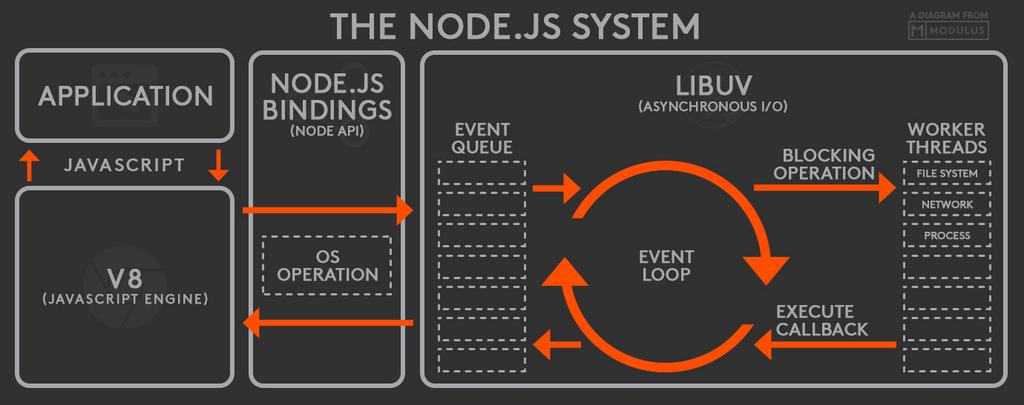
\includegraphics[width=.85\textwidth]{imagem/node-js-system-twitter-BusyRich.png}
    % Caption centralizada
    \captionsetup{justification=centering}
    \captionfont{\small{\textbf{\\Fonte: \cite{nodesystem}}}}	
    \label{fig:node-js-system-loop}
  \end{figure}
  
  A figura \ref{fig:node-js-system-loop} exibe uma síntese do sistema Node.JS. Primeiro a aplicação web requisita um evento 
  ao Node.Js instalado no servidor. Através da linguagem JavaScript V8, o Node.Js interage com sua \ac{API}, e envia 
  a requisição para uma fila que é processada pelo ciclo de eventos e tratada pelos módulos existentes no Node.js. 
  
  Nas próximas seções será explicado ao leitor essas características do ecossistema do Node.Js.
 
\section{JavaScript, Chamadas de retorno e \textit{callback's hell}}
\label{chamadas-de-retorno-e-callback-hell}

  O Node.Js utiliza o JavaScript Engine V8, desenvolvido pela empresa Google, como linguagem de programação
  de sua plataforma utilizando técnicas recentes de compiladores que permitem que o código escrito em linguagem de alto nível,
  tal como o JavaScript, execute de forma semelhante a linguagens de baixo nível como C.  E através do seu alto desempenho, 
  foi possível alterar o contexto de utilização (amplamente utilizada em interfaces de sites nos navegadores) e aplicá-la em 
  servidores Web, formando o ambiente Node.Js.
  
  
  Para o Node.js a linguagem provê nativamente o modelo de eventos assíncronos em operações de entrada e saída, 
  além de suporte a chamadas de retorno, do inglês \textit{callback} \cite{oliveira}.  Ao escrever códigos para a 
  plataforma Node.Js, é necessário ter conhecimento prévio da linguagem JavaScript e a forma como os 
  métodos são implementados com ou sem chamadas de retorno. \cite{hughes}
  
  
%  O JavaScript V8 casou-se muito bem com a orientação a eventos, pois provê nativamente
%  o modelo de eventos assíncronos em operações de entrada e saída, além de suporte à chamadas de retorno.\cite{Oliveira:2012}
  
 
%  Ao escrever códigos em Node.Js é necessário ter em mente que os métodos implementados em JavaScript trabalhe com uma 
%  chamada de retorno de cada vez, para que o programa seja compreensível e também capaz de executar rapidamente várias 
%  tarefas de forma eficiente.\cite{Hughes:2012}

  Essas chamadas de retorno são definidas como uma função especial associada a um determinado evento. Ela tende a ser 
  executada quando o evento é atingido, evitando assim a espera de execução de um processo \cite{wilson}. Por exemplo:
  em um programa JavaScript assíncrono, ao fazer uma requisição a um banco de dados especifica-se na chamada de retorno o 
  que deve ser feito com os resultados do banco de dados. O JavaScript
  não espera a finalização dessa requisição e continua a processar outras atividades existentes no programa. 
  Apenas quando o resultado da requisição é retornado do banco de dados, a lógica implementada na chamada de retorno 
  para manipular os dados é executada \cite{junior}. Ao saber trabalhar com as chamadas de retorno consegue-se aproveitar 
  a performance oferecida pelo JavaScript no Node.Js.
  
  \citeonline{pereira} comparou a execução de dois programas escritos em Node.Js utilizando duas funções nativas
  do módulo (\textit{File System}): \textit{fs.writeFileSync} e \textit{fs.writeFile} para criar 5 arquivos diferentes 
  em um diretório qualquer. A primeira função, \textit{fs.writeFileSync}, utilizando o modelo síncrono, gastou 1000 milissegundos 
  para completar a tarefa. Em contrapartida, a função \textit{fs.writeFile}, utilizando o modelo assíncrono com sua respectiva 
  chamada de retorno, gastou apenas 200 milissegundos até atingir o fim da tarefa. Foram gastos 5 vezes menos tempo utilizando o 
  modelo assíncrono do JavaScript.
  
%  Em resumo, este código é uma repetição de 5 interações e a cada iteração desta repetição é criado um arquivo texto. O primeiro
%  exemplo utiliza o modelo síncrono existente no módulo (\textit{File System}) nativo do Node.Js (\textit{fs.writeFileSync}).
  
%  \begin{figure}[H]
    % Alterar espaçamentos antes e depois do caption
%    \setlength{\abovecaptionskip}{0pt}
%    \setlength{\belowcaptionskip}{0pt}
    % Caption
%    \caption[Tempo de resposta, método síncrono bloqueante]{Tempo de resposta, método síncrono bloqueante}
%    \centering
%    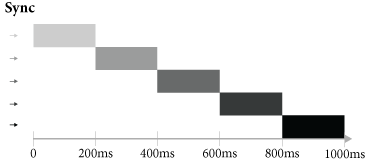
\includegraphics[width=.85\textwidth]{imagem/timeline-node-sync-caio-ribeiro.png}
    % Caption centralizada
%    \captionsetup{justification=centering}
%    \captionfont{\small{\textbf{\\Fonte: \cite{Pereira:2013}}}}	
%    \label{fig:timeline-sync}
%  \end{figure}
  
%  A Figura \ref{fig:timeline-sync} exibe gráfico demonstrando que cada arquivo escrito
%  gasta-se 200 milesegundos totalizando 1000 milesegundos para completar toda a tarefa.

%  O segundo exemplo utiliza o mesmo módulo (\textit{File System}) implementando a função assíncrona. Esta função de acordo com
%  a documentação \cite{ModuleSystemFs:2014} informa que obrigatoriamente precisa passar uma função de chamada de retorno como último
%  parâmetro da função \textit{fs.writeFile}.
 
%  \begin{figure}[H]
    % Alterar espaçamentos antes e depois do caption
%    \setlength{\abovecaptionskip}{0pt}
%    \setlength{\belowcaptionskip}{0pt}
    % Caption
%    \caption[Tempo de resposta, método assíncrono não-bloqueante]{Tempo de resposta, método assíncrono não-bloqueante}
%    \centering
%    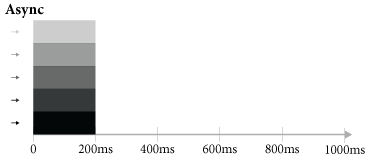
\includegraphics[width=.85\textwidth]{imagem/timeline-node-async-caio-ribeiro.png}
    % Caption centralizada
%    \captionsetup{justification=centering}
%    \captionfont{\small{\textbf{\\Fonte: \cite{Pereira:2013}}}}	
%    \label{fig:timeline-async}
%  \end{figure}

%  A Figura \ref{fig:timeline-async} mostra o gráfico do tempo total de duração para escrever em 05 (cinco) arquivos. Essa 
%  performance é dada a execução assíncrona que maximizou o processamento reduzindo o tempo total para 200 milesegundos.
  
  Apesar da boa performance oferecida pelo modelo assíncrono e as chamadas de retorno, é necessário ficar
  atento às diversas chamadas de retorno encadeadas umas nas outras no processo de desenvolvimento \cite{pereira}. 
  Em complemento, é necessário ter em mente que os métodos implementados trabalham com uma 
  chamada de retorno de cada vez, para que o programa seja compreensível e também capaz de executar rapidamente várias 
  tarefas de forma eficiente\cite{hughes}. Este encadeamento de chamadas de retorno é denominado pelo termo \textit{callbacks hell} 
  e dificulta a manutenibilidade e a legibilidade do código, podendo ocorrer perda de controle do que está sendo executado e acesso às 
  variáveis devido a trocas de escopos. \cite{pereira}
  
  Através de um outro programa (\ref{leitura-arquivos-diretorio-node}) implementado por \citeonline{pereira} e referenciado no 
  Anexo \ref{primeiro-anexo}, uma simples leitura de arquivos de um diretório qualquer, imprimindo o nome e o tamanho em bytes do arquivo 
  pode ser custosa ao desenvolvedor. Neste momento o autor questiona a organização deste código (\ref{leitura-arquivos-diretorio-node}) escrito caso a solução do 
  problema fosse mais complexa. Dando a entender que tal código seria um caos.
  
%  Também é afirmado, que, a linguagem JavaScript por ser assíncrona resulta em ganhos de 
%  performace, porém de perde-se o controle do que está sendo executado, e o acesso à variáveis devido às trocas de escopos
%  neste emaranhado de chamadas de retorno.
  
  Uma das maneiras de se evitar o \textit{callback hell}, uma vez que é uma boa prática de codificação JavaScript, é
  criar funções que expressem seus objetivos de forma isoladas, salvando os retornos em variáveis e passando-as em outras
  chamadas de retorno como parâmetros. A organização do código pode ser visto no código (\ref{leitura-arquivos-diretorio-node-callback-heaven}) do
  Anexo \ref{primeiro-anexo} \cite{pereira}.
 
  Outra abordagem, utilizada pela empresa StrongLoop, é a utilização do módulo async \footnote{Módulo ASYNC, disponível em: https://github.com/caolan/async},
  o mais popular entre os desenvolvedores e que fica mais próximo do \textit{core} (núcleo) do Node.Js. Este módulo
  possui o método \textit{async.waterfall} que provê um controle em série, em que os dados podem ser passados para a próxima função
  usando o parâmetro \textit{next}. O método \textit{async.map} executa o comando \textit{fs.stat} (buscar status do arquivo) do Node.Js sobre uma matriz
  de caminhos, em paralelo. Em seguida retorna uma matriz com a ordem mantida dos resultados. Como dito pela empresa
  Strongloop, este módulo garante que somente uma chamada de retorno será retornada, haverá propagação de erros e controle do 
  paralelismo automaticamente. 
  
  Sobre a propagação de erros, uma observação importante na documentação do módulo \textit{File System} e que 
  vale para todo o ambiente Node.Js e seus módulos, é que os parâmetros passados para a chamada de retorno dependerá da 
  implementação de cada método. Em regra, o primeiro argumento é sempre reservado para uma variável de erro ou exceção 
  que deverá ser tratada no escopo interno da chamada de retorno. Se a operação foi concluída com êxito, o primeiro argumento 
  será nulo ou indefinido, não sendo necessário qualquer tipo de tratamento \cite{modulesystemfs}.
  
  Outro módulo apresentado pela empresa Strongloop é a utilização de \textit{Promises} que fornece tratamento de erros
  e as regalias da programação funcional. Para tal, é necessário utilizar o módulo Q \footnote{Módulo Q, disponível em:https://github.com/kriskowal/q}
  que através do método \textit{q.all} executa todas as chamadas de status dos arquivos em paralelo e em seguida retorna uma matriz
  com a ordem dos dados mantidas. 
  
  Ao contrário de exemplos anteriores, quaisquer exceções são lançadas dentro da cadeia dos
  \textit{promises}. Somente depois tais exceções são capturadas e manipuladas.
  Por fim, como descreve \citeonline{strongloop}, existe a abordagem utilizando \textit{generators} que estarão
  contemplados e integrados oficialmente em versões posteriores à 0.11.2 do Node.Js. Os \textit{generators} podem ser definidos
  como co-rotinas para o JavaScript e permitem que uma função possa ser suspensa e retornada
  utilizando a palavra reservada \textit{yield}. Ao utilizar o módulo CO é possível manipular erros (incluindo exceções levantadas)
  serão passadas para a função de chamada de retorno. Também é habilitado o uso de blocos \textit{try/catch} em torno das 
  declarações \textit{yield}.
  
  Em seu artigo, \citeonline{strongloop} investigou três possibilidades de mitigar o problema dos \textit{callbacks hell}, com o 
  intuito de obtenção de controle do fluxo da aplicação. Um interesse maior surgiu pela abordagem dos \textit{generators},
  apesar de não empregar em seus projetos. Independente de qual módulo e abordagem for utilizada a empresa Strongloop reafirma que é recomendado
  utilizar a modularização em qualquer parte da aplicação e das bibliotecas descritas (\textit{async,promises, generators}).
  
  Após breve entendimento da linguagem JavaScript e aproveitadas pelo Node.Js, descreve-se na próxima seção
  o paradigma de orientação a eventos que compõe a plataforma Node.Js.
  
  
\section{Programação Orientada a Eventos}
\label{programacao-orientada-a-eventos}

  
  As aplicações desenvolvidas em Node.Js têm como núcleo e referência os eventos. Estes eventos são indicações de que ocorreu algo, 
  havendo dois atores para este modelo de programação \cite{oliveira}. Utilizando a terminologia de produtor do evento, 
  do inglês \textit{event producer} e o consumidor do evento, do inglês \textit{event consumer}, identifica-se estes dois atores. 
  Uma característica deste modelo de programação é que o produtor do evento não espera pela ação a ser executada  pelo servidor. 
  Em contrapartida, os servidores Web tradicionais utilizam o conceito de ação e resposta e esperam por uma resposta \cite{junior}.
  
  \citeonline{pereira} compara a orientação de eventos do Node.Js à filosofia de orientação 
  de eventos utilizada nos navegadores; a diferença entre elas é que no Node.Js 
  não existem eventos de clique do mouse, teclas pressionadas do teclado, do inglês \textit{keyup}, ou qualquer evento de componentes HTML. 
  Mas há operações de entrada e saída do servidor: eventos de conexão ao banco de dados, abertura de arquivo e \textit{streaming}
  de dados. Em complemento a esta abordagem o Node.Js inicia seu objetivo de criar aplicações de rede escaláveis, utilizando \textit{thread} única
  e o ciclo de eventos para resolver os gargalos de altas conexões.

\section{Única thread e o ciclo de eventos}
\label{single-thread}

  Uma \textit{thread} pode ser conceituada como um conjunto de instruções executadas pelos processos do sistema operacional.
  Sendo que cada thread é um fluxo diferente de controle que pode executar estas instruções de forma independente, em exemplo,
  uma thread pode executar o GUI, enquanto uma segunda instrução faz algumas operações de entrada e saída, 
  enquanto um terceiro executa cálculos. \cite{lewis}
  
  Em Node.Js as conexões são recebidas em uma única \textit{thread} invocada pelo nó de servidor de processos, do inglês \textit{node server process}.
  \citeonline{abernethy} cita que em vez de criar \textit{threads}
  no sistema operacional para cada conexão e alocar a memória RAM que acompanha essas \textit{threads}, 
  cada conexão dispara um evento executado no processo do motor Node.Js.   
  \citeonline{powers} cita também a \textit{thread} única como um dos benefícios do ambiente do Node.Js, 
  pois o aplicativo pode ser facilmente escalável uma vez que em um único segmento de execução não há sobrecarga 
  de requisições. Citando o exemplo de seu livro, em um sistema web desenvolvido em \ac{PHP} e em Node.Js com os mesmos requisitos
  não haverá diferenças para o usuário final do aplicativo, pois visualizariam as mesmas páginas. Porém ao investigar 
  os processos no servidor é possível constatar uma diferença entre as duas aplicações.
  
  Com o \ac{PHP} e o servidor web Apache, cada pedido que for solicitado abrirá um processo filho do Apache. O que não ocorre 
  com o Node.Js, pois sua execução é em \textit{thread} única.  Caso o servidor web Apache for pouco otimizado, a sua capacidade 
  de criar processos filhos restringe-se a um par de centenas de processos filhos em paralelo. Se a porventura a quantidade 
  de usuários do sistema web em \ac{PHP} for maior que capacidade de criar os processos filhos do Apache, o cliente entrará 
  numa fila e esperar por uma resposta \cite{powers}.

  Assim como \citeonline{powers}, \citeonline{hughes} afirmam que o conceito de \textit{thread} única é importante para 
  toda a plataforma do Node.Js. Porém, uma das críticas feitas ao Node.Js pela comunidade de desenvolvedores 
  é que utilizando este conceito, não é possível realizar concorrência no servidor de processos.
  
  \citeonline{pereira} enfatiza que não é possível trabalhar com programação 
  concorrente em plataforma multi \textit{thread} nativamente com o ambiente Node.Js. Mas existem maneiras de implementar sistemas concorrentes, 
  como por exemplo a utilização de \textit{clusters}, o qual é um módulo nativo do ambiente Node.Js.
  
  Através de outra biblioteca, \textit{multi-node} \citeonline{zyp}, é possível compartilhar \textit{sockets} nos servidores.
  Desta maneira o nó de servidor de processos pode ser instanciado em um ou mais processadores, oferecendo paralelismo, 
  atendendo e recebendo requisições na mesma porta. Cabendo ao sistema operacional atuar como balanceador de carga.\cite{oliveira}
  
  Com a \textit{thread} única é possível suportar um alto número de conexões, em conjunto com a repetição implícita existente no Node.Js. 
  Essa repetição é denominada de ciclo de eventos, do inglês \textit{event loop}, e tem como função esperar os eventos e repassá-los 
  ao manipulador de eventos \cite{tilkov}.
  O ciclo de eventos é uma repetição infinita que a cada interação verifica em sua 
  fila de eventos se um determinado foi emitido ou se existem novos. Estes eventos só aparecem na 
  fila quando são emitidos durante as suas interações na aplicação; quando ocorre, é emitido um evento, então este
  é executado e enviados para a fila de executados \cite{pereira}.
  Intuitivamente o ciclo de eventos é similar à vida cotidiana, pois cada solicitação de evento necessita de um retorno.
  
%  \citeonline{Pereira:2013} diz que a programação orientada a eventos do Node.Js 
%  foi inspirado pelos \textit{frameworks} Event Machine\footnote{http://rubyeventmachine.com/} do 
%  Ruby\footnote{https://www.ruby-lang.org/en/} e Twisted\footnote{https://twistedmatrix.com/trac/} do 
%  Python\footnote{https://www.python.org/}, porém o ciclo de eventos do Node.Js é mais perfomático pois seu mecanismo 
%  é nativamente executado de forma não bloqueante sendo o diferencial em relação a outros ambientes de programação.
  
%  \citeonline{Wilson:2013} enaltece os eventos do Node.Js, fornecido pelo JavaScript. Em outras linguagens de programação 
%  os fluxos de trabalho são em \textit{threads} múltiplas e concorrentes, sendo que cada \textit{thread} gasta a maioria de seu tempo aguardando 
%  operações bloqueadoras de entrada e saída, tais como: leitura ou escrita em disco, manipulação do banco de dados 
%  acesso a informações pela rede. O que não ocorre com o Node.Js.
   

  
%  Possuindo a base de como o ciclo de eventos funciona, o desenvolvedor é capaz de usá-lo em toda sua potencialidade, 
%  conseguindo vantagens e evitando armadilhas dessa abordagem.\cite{Hughes:2012}
  
  Aprofundando, \citeonline{pereira} cita o módulo \textit{EventEmitter} como responsável por emitir esses eventos e em 
  grande maioria das bibliotecas existentes no Node.Js utilizam as funcionalidades de eventos deste módulo. 
  No processo de execução do evento pode-se programar qualquer lógica de programação através do 
  mecanismo de chamada de retorno. Tal chamada de retorno pode ser executada através de uma função de escuta, 
  semanticamente conhecida pelo on().
  
  Essa seção é melhor descrita e exemplificada por \citeonline{wilson} 
  em seu livro que nos mostra o uso e o desenvolvimento destes eventos com o módulo \textit{Event Emitter}.
  Através deste paradigma empregado no Node.js, a aplicação pode 
  suportar dezenas de milhares de conexões simultâneas. Os bloqueios ou impasses não são características da plataforma ao
  realizar processamento de entradas e saídas devido a orientação a eventos. \cite{abernethy}
  O único gargalo de um servidor Node.Js passa a ser a capacidade de tráfego da aplicação.\cite{oliveira} 


\section{O framework Express.Js}
\label{framework-express}

  \citeonline{powers} explica que um \textit{framework} ajuda na infraestrutura e nos permite criar sites e aplicações
  com agilidade, fornecendo ao desenvolvedor um esqueleto capaz de oferecer um suporte no processo de desenvolvimento de
  software. Com os \textit{frameworks}, o foco é a criação de funcionalidades da nossa aplicação ou site e 
  também fornece coesão ao código, o que nos beneficia com legibilidade e manutenibilidade.

  \citeonline{pereira} complementa que utilizar a API HTTP nativa do Node.Js pode ser um processo moroso e desgastante
  para o desenvolvedor. 
  Com o surgimento de novas necessidades de implementação e o acréscimo de novas funcionalidades,
  os códigos se tornarão gigantescos, aumentando a complexidade do projeto e dificultando futuras manutenções. Assim surge o 
  \textit{framework} Express.Js, para solucionar necessidades e agilizar o desenvolvimento.
  
  \citeonline{powers} compara o \textit{Express.Js} ao \textit{framework} Sinatra \footnote{Framework escrito em Ruby para criar aplicações Web. 
  Disponível em http://www.sinatrarb.com/intro.html} sendo o primeiro bem mais \textit{RESTFUL}. 
  Pereira(2012) reafirma e complementa que o módulo \textit{Express.Js} foi inspirado pelo \textit{framework} Sinatra da 
  linguagem Ruby e que é bastante utilizado em aplicações web de grande escala.
  
  Suas características são descritas por \citeonline{pereira}:
  
  \begin{compactitem}
    \item[a)] Modelo, visão e rotas;   
    
    \item[b)] Modelo, visão e controladores;
    
    \item[c)] Roteamento de URL's com chamadas de retorno;
    
    \item[d)] \textit{Middleware};
    
    \item[e)] \textit{Interface} REST;
    
    \item[f)] Suporte a \textit{upload} de arquivos.
    
    \item[g)] Configuração baseada em variáveis de ambiente;
    
    \item[h)] Suporte a \textit{helpers} dinâmicos;
    
    \item[i)] Integração com \textit{Templates Enginies};
    
    \item[j)] Integração com \ac{SQL} e \ac{NoSQL};
    
  \end{compactitem}
  
  Ao criar um esqueleto utilizando o \textit{Express.js} é importante ter conhecimento do que cada
  arquivo ou diretório representa. \citeonline{powers, hughes} não apresentam um descritivo de cada arquivo 
  ou diretório e seu papel. \citeonline{pereira, wilson} tratam mais deste assunto, o que pode ser visto
  no apêndice \ref{apend:express-skel}.
  
\subsection{O servidor web com \textit{Express.Js}}
\label{servidor-web-express-js}

  
  De acordo com \citeonline{wilson}, o interessante do Node.Js é que o código do 
  programa que se escreve para ele também é a implementação do servidor: 
  Seguindo este modelo se tem a expectativa de que a aplicação funcione e se comporte de modo semelhante 
  ao ambiente de produção assim como no desenvolvimento, pois não existe nenhuma biblioteca, nenhum intermediário 
  ou \textit{daemon} que esteja no caminho.
  
  O arquivo \textit{app.js} criado pelo \textit{Express.js} é pequeno mas com grandes funcionalidades inclusas, como 
  roteamento para solicitações entrantes do \ac{HTTP}, motores de visões para renderizar marcações do HTML5
  e também download dos arquivos estáticos.